\documentclass[twocolumn]{article}
\usepackage[utf8]{inputenc}
\usepackage[T1]{fontenc}
\usepackage[margin=1in]{geometry}
\usepackage{graphicx}
\usepackage[font=small,labelfont=bf]{caption}
\setlength{\columnsep}{0.3in}
\title{Kilonovaen og oprindelsen af guld}
\author{Jonatan Selsing \\
	The Cosmic Dawn Center \\
	 Niels Bohr Instituttet  \\
	 Københavns Universitet \\
	}

\date{\today}
% Hint: \title{what ever}, \author{who care} and \date{when ever} could stand 
% before or after the \begin{document} command 
% BUT the \maketitle command MUST come AFTER the \begin{document} command! 
\begin{document}

\maketitle


\begin{abstract}
I denne her artikel vil jeg introduce et fænomen som for nyligt er trådt frem på den astronomiske scene. Kilonovaen har vist sig at være ét af de mest eksotiske, sjældne, og samtidig betydningsfulde begivenheder der sker i universet. En kilonova er et resultat af sammenstødet mellem to neutronstjerner, eller en neutronstjerne og et sort hul. I sammenstødet bliver neutron-stjerne materiale slynget ud i universet, og dette materiale bliver til alle de tungeste grundstoffer vi kender, som bla. gulv, sølv og platin. 
\end{abstract}

\section{Introduction}
Den 17. august 2017 skete der noget specielt i de tre tyngebølgedetektorer der udgør LIGO/Virgo samarbejdet. For første gang registrerede detektorerne det karakteristiske "tyngdebølge-skvulp" fra et binært system, hvis vægt begrænset til ca. 2.8 somasser og derfor konsistent med to neutronstjerner \cite{abbotta}. Uafhængigt, og forsinket med 1.7 s, detekterede GBM (Gamma-ray Burst Monitor) instrumentet ombord rum-teleskopet \textit{Fermi}, et kort signal af gamma-stråler, konsistent med den type signal vi kender fra korte gamma-glimt. Derfra vidste vi med det samme, at tyngdebølgesignalet rejste sammen med noget elektromagnetisk stråling, hvilket betød, at vi for første gang i verdenshistorien havde muligheden for at se det optiske modstykke til et tyngdebølgesignal. Dette optiske modstykke var på forhånd teoretiseret til at være lysstrækt nok til, at vi ville kunne se det, samt potentielt selt set være kilden til alle de tungeste grundstoffer i universet \cite{lattimer}. På grund af formodningen om betydningen af at finde dette modstykke, var det virkeligt vigtigt at sikre en hurtig opfølgning med teleskoper, inden det optiske lys blev for svagt til se mere. 

Ved at triangulere på baggrund af ankomst-tidspunktet af signalet i tyndebølgedetektorerne kunne vi finde frem til, at dette her sammenstød skete over den sydlige halvkugle, inden for et område på størrelse med fuldmånen, hvilket er ca 28 kvadratgrader. Dette lyder måske ikke af meget, men en typisk størrelse et teleskop dækker omkring  0.25 kvadratgrad, så det kræver alligevel en del enkelte pointings at dække hele området. 

Mellen omdragelsen af kilonovaen og offentliggørelsen, blev Rainer Weiss, Barry C. Barish og Kip S. Thorne tildelt Nobelprisen i fysik for opdagelsen af tyngdebølger. 

\begin{center}
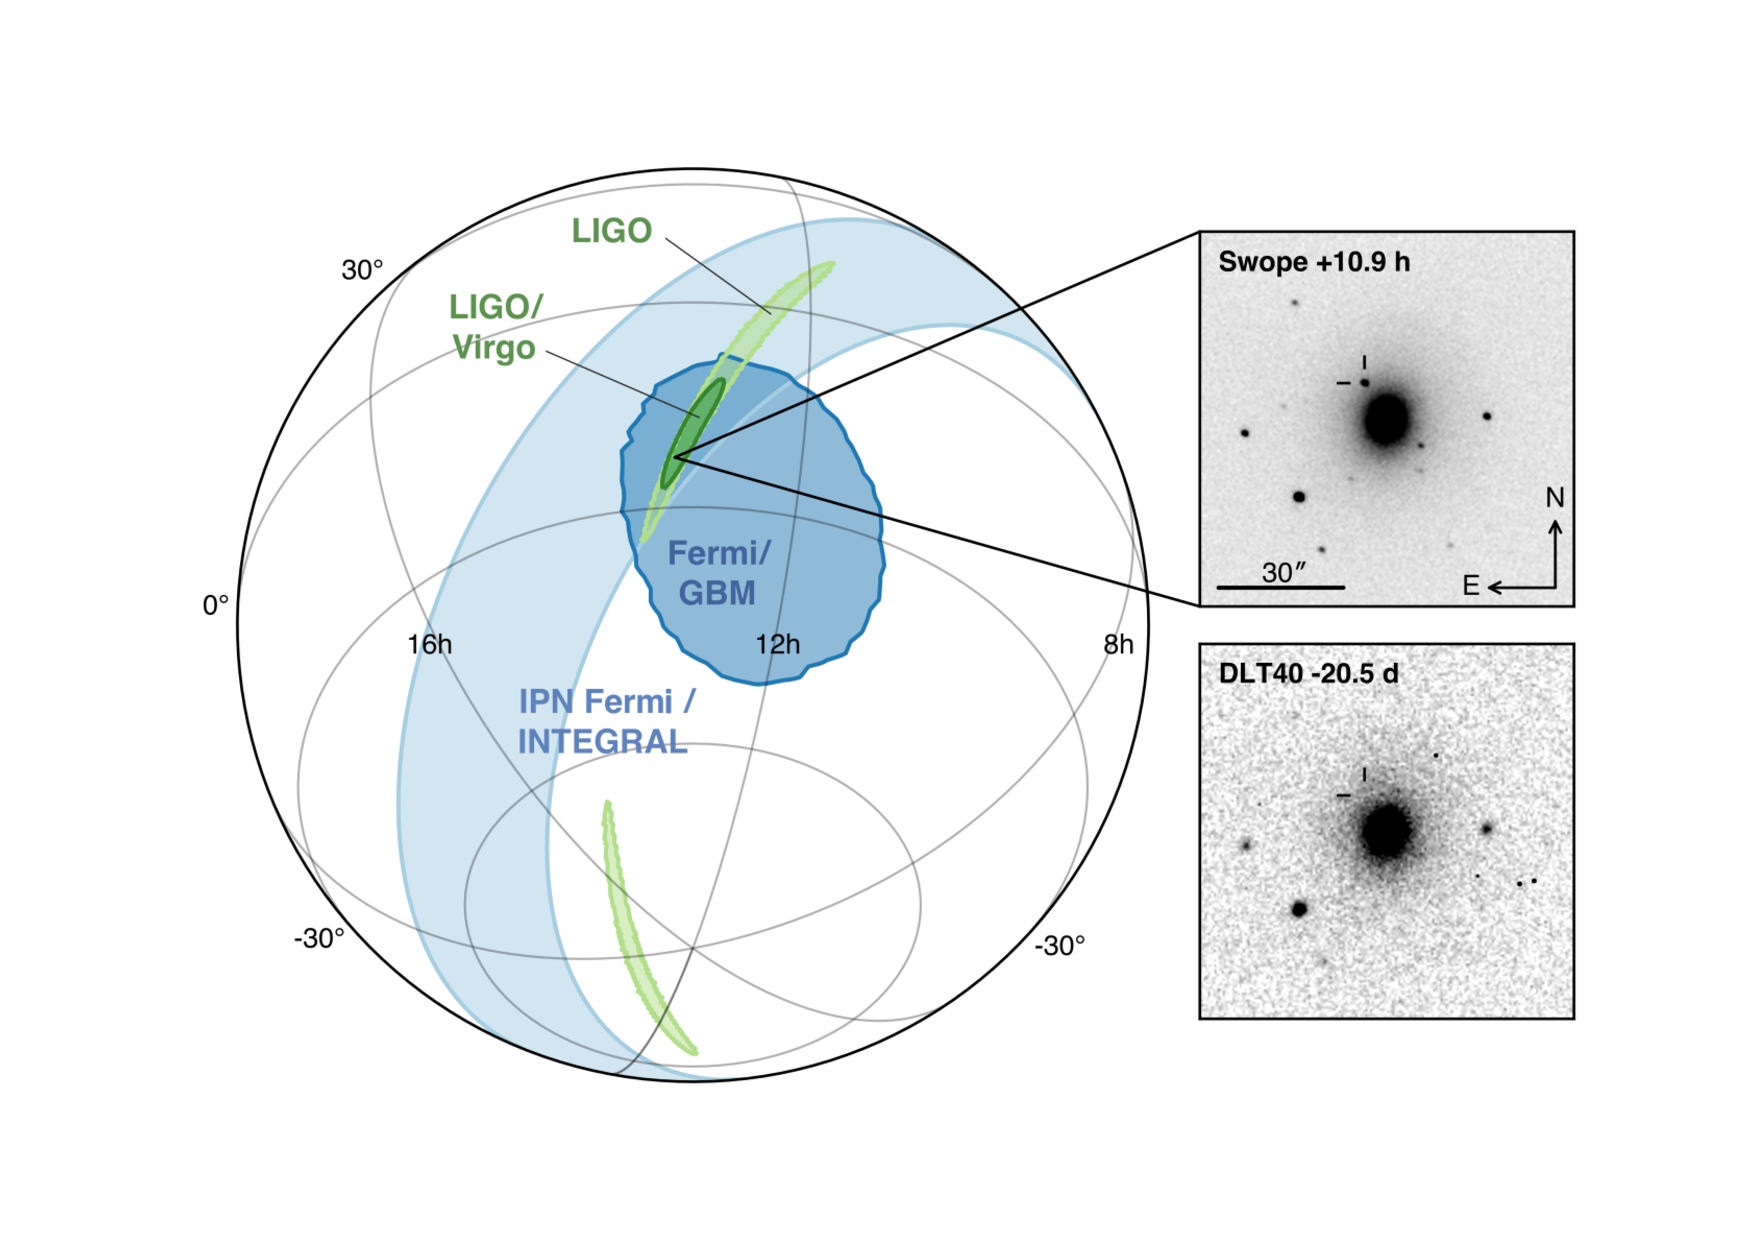
\includegraphics[width=\columnwidth]{GW170817_MMA_Skymap}
\captionof{figure}{Lokaliseringen af kilonovaen baseret på ankomst-tidspunktet af tyngebølgesignet til de forskellige detektorer, samt GBM lokalisationen. Figuren er  fra \cite{abbottb}}
\end{center}








\section{Conclusions}\label{conclusions}




\begin{thebibliography}{9}
\bibitem[1]{abbotta} \emph{GW170817: Observation of Gravitational Waves from a Binary Neutron Star Inspiral.},
B. P. Abbott, et al., Physical Review Letters 119, 161101 (2017).

\bibitem[1]{abbottb} \emph{Multi-messenger Observations of a Binary Neutron Star Merger.},
B. P. Abbott, et al., The Astrophysical Journal Letters, 848:L12 (2017).

\bibitem[2]{lattimer} \emph{Black-hole-neutron-star collisions.},
Lattimer, J. M. \& Schramm, D. N., The Astrophysical Journal Letters 192:L145 (1974).
\end{thebibliography}

\end{document}
